\documentclass[border=6pt]{standalone}

\usepackage{tikz}
\usetikzlibrary{positioning, arrows.meta}

\definecolor{otblue}{HTML}{0072B2}
\definecolor{otorange}{HTML}{E69F00}
\definecolor{otteal}{HTML}{009E73}
\definecolor{otpurple}{HTML}{CC79A7}
\definecolor{otgray}{HTML}{5A5A5A}

\begin{document}
% ==== parameters (edit these) ============================================
\def\eonelabel{T0\\Setup}
\def\etwolabel{T1\\Train}
\def\ethreelabel{T2\\Eval}
\def\efourlabel{T3\\Ablate}
\def\efivelabel{T4\\Write}
% =========================================================================

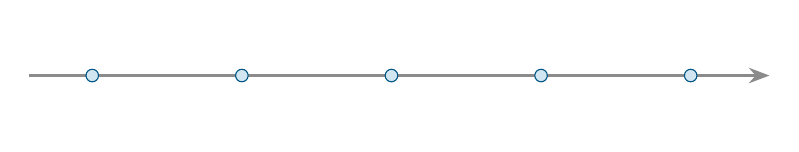
\begin{tikzpicture}[
  >={Stealth[length=2.6mm]},
  axis/.style={draw=otgray!70, line width=1.15pt, ->},
  tick/.style={circle, draw=otblue!75!black, fill=otblue!18, inner sep=1.6pt},
  aboveevent/.style={font=\sffamily\footnotesize, align=center, text=otgray!20!black},
  belowevent/.style={font=\sffamily\footnotesize, align=center, text=otgray!20!black},
]
  \draw[axis] (0,0) -- (9.4,0);
  \foreach \x/\name/\side in {
    0.8/e1/above,
    2.7/e2/below,
    4.6/e3/above,
    6.5/e4/below,
    8.4/e5/above
  }{
    \node[tick] (\name) at (\x,0) {};
  }
  \node[aboveevent, above=0.28cm of e1] {\eonelabel};
  \node[belowevent, below=0.28cm of e2] {\etwolabel};
  \node[aboveevent, above=0.28cm of e3] {\ethreelabel};
  \node[belowevent, below=0.28cm of e4] {\efourlabel};
  \node[aboveevent, above=0.28cm of e5] {\efivelabel};
\end{tikzpicture}
\end{document}
